\clearpage
\begin{flushright}
    \textit{Лекция №15}
    \textit{2015.11.03}
\end{flushright}

Как только другой процесс вызовет receive(), процесс, пославший сообщение, будет разблокирован. Он будет заблокирован, пока не будет обработан и не вызван replay().

\chapter{Средство межпроцессного взаимодействия Unix}
Синхронизация – связь между процессами, при котором один процесс не может выполняться, начиная с определенного места до тех пор, пока другой процесс не достигнет своей определенной точки. Пример: один процесс записывает данные в буфер. Оба процесса должны быть синхронизированы.

IPC (средство межпроцессного взаимодействия Unix). 

\section{Сигналы}

Соответствуют определенным событиям в системе. Механизм сигналов позволяет процессам реагировать. Получение некоторым процессом сигнала означает завершиться. Реакция процесса на принимаемый сигнал зависит от того, как процесс определил свое поведение. У процессов есть для этого сигнальные маски. Потомок – наследует сигнальную маску.

Системный вызов \verb|int kill(int pid, int sig)|. Если процесс вызовет \verb|kill(getpid(), sigalarm)| – будет подан сигнал этому же процессу. 
Системный вызов \verb|void (*signal(int sig, void (*handle)(int)))(int)| – реакцией на сигнал будет вызов \verb|handle|. Сигналы посылаются группе процессов. При это в зависимости от определенных значений в параметрах в соответствующих вызовов может быть разный состав групп, но вообще это процесс, вызвавший многократно \verb|fork| создает группу (подчинение сверху вниз). Предок – создатель группы процессов. Т.е. процессы родственники могут получать в системе одни и те же сигналы. Важнейший сигнал – уничтожение процесса. Системный вызов сигнал возвращает сигнал на предыдущий обработчик данного сигнала в результате его можно использовать для восстановления обработчика сигнала, написав следующее:

\begin{figure}[H]
    \centering
    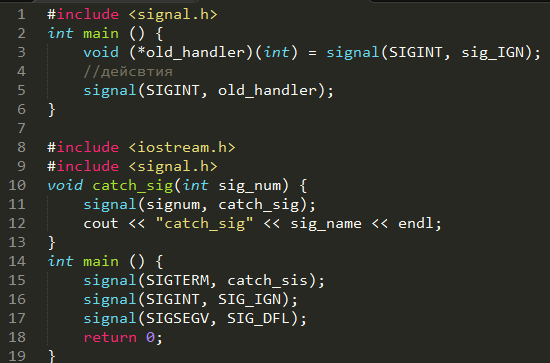
\includegraphics[width=\textwidth]{listing/2.png}
    \caption{listing}
\end{figure}

Перехват сигнала \verb|SIGTERM|, реакция на \verb|SIGSEGV| должна быть установлена стандартным образом.
Не рекомендуется использовать \verb|signal| при разработке переносимых приложений, так как его поведение в System V отличается от поведения в BSD. POSIX – portable operating system interface based on unix – интерфейс переносимых ОС. 
POSIX.1 FIPS – федеральный американский стандарт. В BSD – классическое средство взаимодействия – сокеты.
В Европе разработан x/open portability Cuide (XPG3, XPG4) для разработки переносимого ПО. Содержат POSIX 1, POSIX 2, ANSI C. 
В POSIX определены системные вызовы SING LONG JUMP (получив определенный сигнал можно перейти в определенную точку ПО). 

\section{Семафоры}

Unix поддерживают наборы считающих семафоров. Доступ к отдельному семафору – по индексу. Первый семафор – нулевой индекс. Семафоры в системе поддерживаются таблицей семафоров в ядре, одна на систему. В этой таблице отслеживаются все создаваемые в системе наборы семафоров. 

Каждый дескриптор содержит следующие данные о наборе семафоров: 
\begin{enumerate}
    \item имя (целое число, присваивается процессом, который создал набор). Другие процессы по этому имени могут открыть набор и получить дескриптор, чтобы получить доступ.
    \item UID (создателя набора и идентификатор его группы, процесс может удалять набор и изменять управляющие параметры, если его UID совпадает с UID в дескрипторе семафора)
    \item права доступа (для user, group, others)
    \item кол-во семафоров в наборе
    \item последнее время обращения
    \item время последнего изменения управляющих параметров набора
    \item указатель на массив семафоров.
\end{enumerate} 

Операции над набором семафоров:
\begin{enumerate}
    \item \verb|semget()| - создания семафоров;
    \item \verb|semetl()| - изменение параметров;
    \item \verb|semop()| - изменение состояние.
\end{enumerate} 

\begin{figure}[H]
    \centering
    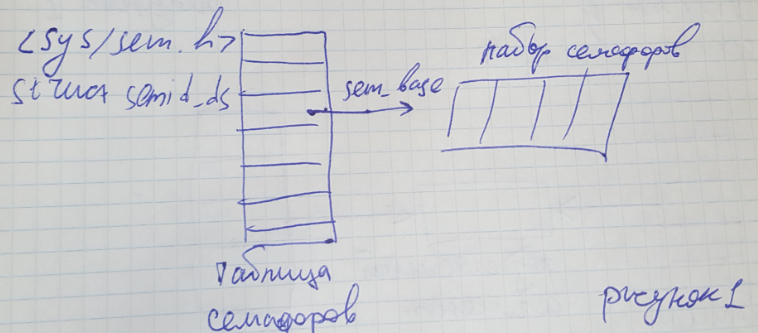
\includegraphics[width=\textwidth]{pic/3.png}
    \caption{pic}
\end{figure}

\begin{lstlisting}[language=c, caption = Структура $semid\_ds$]
struct semid_ds {
	ushort sem_index;
	short sem_op;
	short sem_fe;
}
\end{lstlisting}

На семафорах определены три операции (в отличие от семафоров Дейкстры):
\begin{enumerate}
    \item \verb|sem_op > 0| – инкремент - освобождает ресурс
    \item \verb|sem_op = 0| – проверка освобождения ресурса без попытки захвата
    \item \verb|sem_op < 0| – декремент – захват ресурса
\end{enumerate} 

\begin{figure}[H]
    \centering
    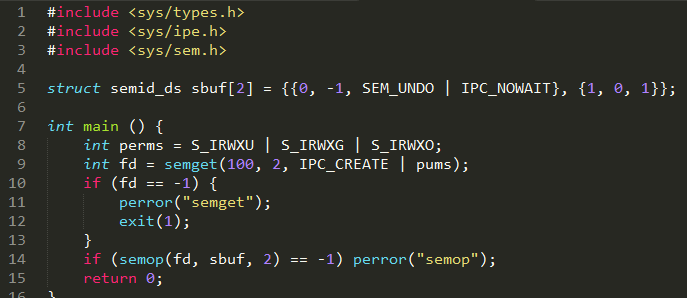
\includegraphics[width=\textwidth]{listing/3.png}
    \caption{Демонстрируем работу набора семафоров}
\end{figure}

Для всех категорий пользователей устанавливаются полные права. Если cистемный вызов \verb|semget()| выполнился успешно, то процесс вызывает системный вызов \verb|semop()|, который передает массив структур \verb|sbuf|, каждая структура определяет действие на одном семафоре наборе. На первом семафоре – декремент, на втором – проверяется на ноль. На семафорах допустимо использовать специальные флаги \verb|IPC_NO_WAYT| – информирует ядро о нежелании процесса переходить в состояние ожидания. Наличие флага объясняется желанием избежать блокировки всех процессов в очереди к семафору, если захвативший семафор процесс завершится аварийно или получит сигнал \verb|KILL|, который перехватить нельзя. В результате уничтожаемый процесс не сможет осуществить освобождение семафора.  И если не предпринять соответствующих мер, то все ожидающие будут заблокированы навечно. \verb|SEMONDO| – указывает ядру, что необходимо отслеживать изменения значения семафора операцией \verb|semop|. И при завершении процесса система ликвидирует сделанные изменения, чтобы процессы небыли заблокированы навечно.

\section{PIPE Программные каналы}

Существуют программные каналы двух типов: именованные и не именованные. Поддерживаются, как специальные файлы.

\begin{enumerate}
    \item неименованные: не имеют идентификатора. Имеют дескриптор. Ими могут пользоваться только процессы родственники, так как при fork наследуются дескрипторы всех открытых файлов.
    \item именованные – имеют имя.
\end{enumerate} 

Программный канал является буфером в системной области памяти. Труба буферизуется на трех уровнях:
\begin{enumerate}
    \item В системной области памяти.
    \item В файловой системе помечается буквой p
    \item При переполнении системной памяти, буферы, имеющие большое время существования, переписываются на диск, при этом используются стандартные функции работы с файлами. Если процесс пытается записать больше 4096 байт, то труба буферизуется во времени.
\end{enumerate} 


\section{Файлы, отображаемые в памяти}

Связано с механизмом одноуровневой памяти. Рассмотрели схемы управления виртуальной памяти, наличие на диске специальной области свопинга. Туда вытесняются страницы из оперативной памяти. 

Один и тот же файл может находить в системе в трех копиях:
\begin{enumerate}
    \item оперативной памяти;
	\item области свопинга;
	\item файловая система.
\end{enumerate} 

Если осуществлять свопинг в область адресного пространства файла, то дополнительная область свопинга не нужна. Этот подход был реализован в системе AS400/OS400 \cite{Soltis_AS400}. Этот механизм получил называние – файлы, отображаемые в памяти. В Windows экзешники выполняются, как файлы, отображаемые в памяти.